\chapter{Metodika a vlastní řešení}

\section{Architektura systému}

Systém LifeMeter se skládá ze dvou hlavních součástí: mobilního klienta a~serverové
části nasazené v~cloudovém prostředí. Mobilní klient komunikuje se serverem za použití
REST API přes protokol HTTPS. Celkové uspořádání systému je znázorněno
na obrázku~\ref{fig:system-overview}.

\begin{figure}[htbp]
    \centering
    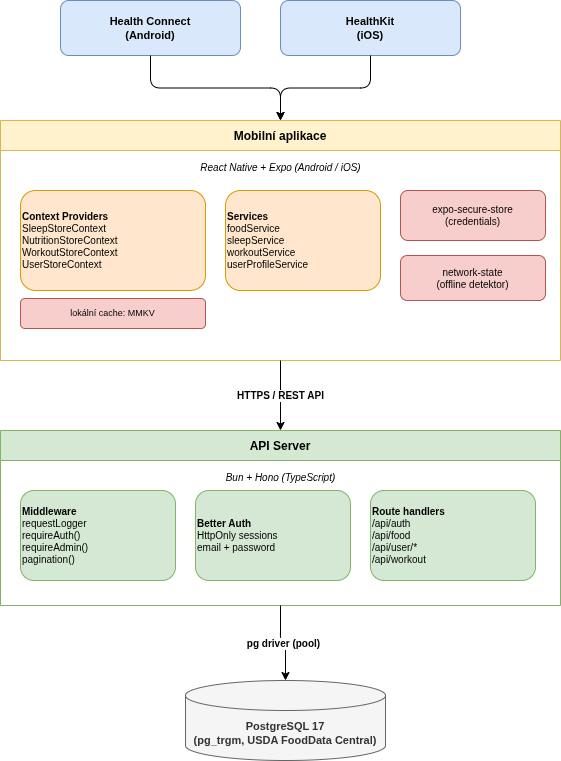
\includegraphics[width=0.92\textwidth]{asset/diagrams/system_overview.png}
    \caption{Přehled architektury systému LifeMeter}
    \label{fig:system-overview}
\end{figure}

\subsection{Klientská vrstva}

Mobilní aplikace je vyvinuta pomocí frameworku React Native ve spojení s~platformou
Expo~\cite{expo}, která zajišťuje přenositelnost mezi operačními systémy Android a~iOS
z~jedné sdílené kódové základny. Na platformě Android jsou zdravotní data čtena přes
rozhraní Health Connect~\cite{healthconnect2024}, na platformě iOS pak prostřednictvím
HealthKit~\cite{healthkit2024}.

Aplikační stav je spravován čtveřicí doménových Context Providers -- \texttt{SleepStoreContext},
\texttt{NutritionStoreContext}, \texttt{WorkoutStoreContext} a~\texttt{UserStoreContext}.
Každý provider zapouzdřuje data a~operace pro příslušnou doménu a~vystavuje je potomkům
stromu komponent prostřednictvím React Context API. Lokální perzistenci dat zajišťuje knihovna
MMKV~\cite{mmkv2024}: data jsou primárně čtena z~cache v~paměti zařízení a~synchronizována
se serverem při obnovení síťového připojení, v~souladu s~principem \textit{offline-first}~\cite{offlinefirst2015}.
Přihlašovací údaje jsou ukládány šifrovaně prostřednictvím \texttt{expo-secure-store}.

\subsection{Serverová vrstva}

Serverová část je implementována v~prostředí Bun s~využitím webového frameworku
Hono~\cite{hono2024}. Každý příchozí požadavek prochází globálním middlewarovým řetězcem:
\texttt{requestLogger} zaznamenává HTTP provoz, autentizační middleware injektuje informace
o~relaci (\texttt{c.get("user")}) a~\texttt{pagination()} normalizuje parametry stránkování.
Správu uživatelských relací zajišťuje knihovna Better Auth~\cite{betterauth2024} prostřednictvím
stavových \texttt{HttpOnly} cookies, v~souladu s~doporučeními OWASP~\cite{owasp2024mobile}.

Routy jsou organizovány doménově: \texttt{/api/auth} zpracovává přihlášení a~registraci,
\texttt{/api/food} poskytuje přístup k~databázi potravin, \texttt{/api/user/*} sdružuje
endpointy pro spánek, jídla, tréninky a~uživatelský profil a~\texttt{/api/workout}
vystavuje referenční data (cviky, styly sérií). Chráněné routy vyžadují middleware
\texttt{requireAuth()}, administrátorské pak \texttt{requireAdmin()}.

\subsection{Datová vrstva}

Datová vrstva je tvořena relační databází PostgreSQL~17~\cite{postgresql2024}.
Rozšíření \texttt{pg\_trgm}~\cite{pg_trgm2024} umožňuje efektivní trigram-based
fulltextové vyhledávání v~databázi potravin, jejíž obsah pochází z~veřejně dostupného
zdroje USDA FoodData Central~\cite{usda2024}. Serverová část komunikuje s~databází
prostřednictvím connection poolu knihovny \texttt{pg}.

\section{Datový model}

Databázové schéma aplikace LifeMeter je rozdělena do pěti doménových skupin:
autentizace a~správa relací (spravováno knihovnou Better Auth), výživa, spánek,
tréninky a~uživatelský profil. Schéma je implementováno v~PostgreSQL~17 a~je
verzováno prostřednictvím migračních SQL souborů. Entity-relationship diagram
celého schématu je uveden na obrázku~\ref{fig:er-diagram}.

\begin{figure}[htbp]
    \centering
    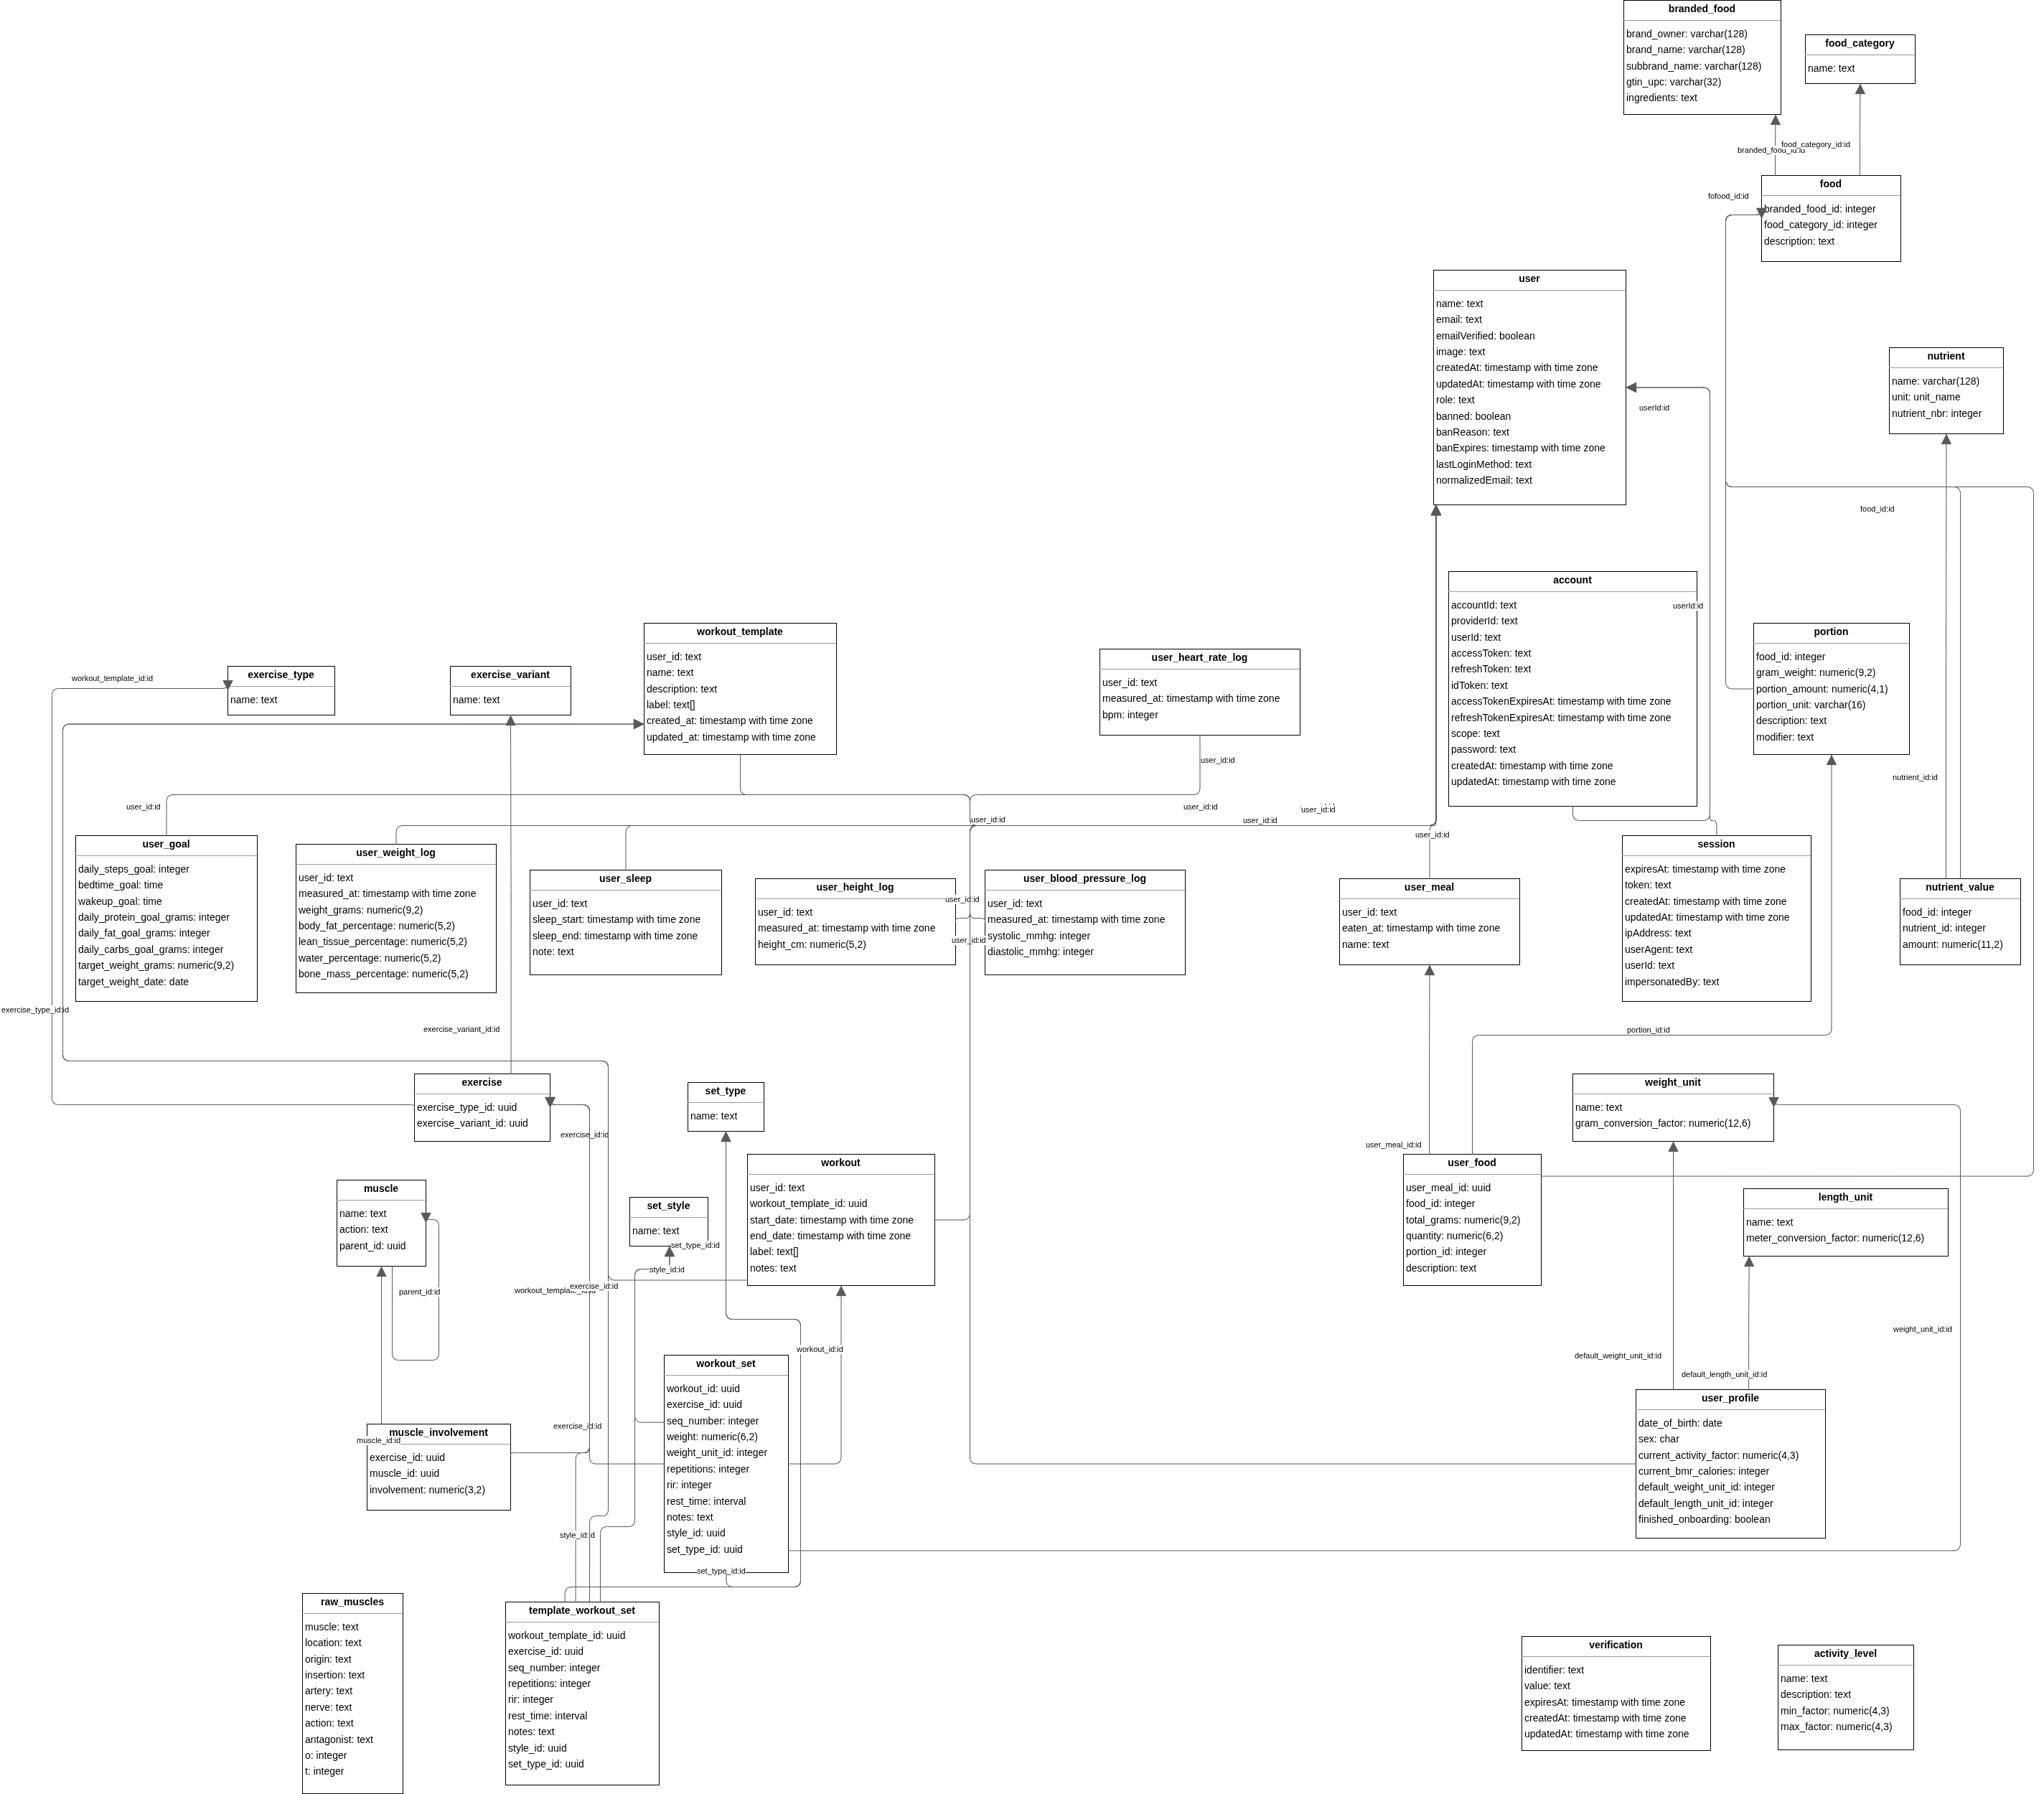
\includegraphics[width=\textwidth]{asset/diagrams/er_diagram.png}
    \caption{Entity-relationship diagram databázového schématu}
    \label{fig:er-diagram}
\end{figure}

\subsection{Autentizace}
Tabulky pro správu uživatelů, relací a ověřování jsou generovány knihovnou Better Auth~\cite{betterauth2024} a~nejsou spravovány vlastními migracemi. Centrální entitou je tabulka \texttt{user}, na kterou jsou pomocí cizích klíčů navázány všechny uživatelské záznamy v~ostatních doménách.
% ==========================================
% Tabulka: user
% ==========================================
\begin{table}[ht!] 
\centering
\begin{tabular}{|l|l|p{7cm}|}
\hline
\textbf{Sloupec} & \textbf{Datový typ} & \textbf{Popis} \\ \hline
id & TEXT & Unikátní identifikátor záznamu \\ \hline
name & TEXT & Celé jméno uživatele \\ \hline
email & TEXT & E-mailová adresa uživatele \\ \hline
emailVerified & BOOLEAN & Příznak, zda byl e-mail uživatele ověřen \\ \hline
image & TEXT & Odkaz na profilový obrázek uživatele \\ \hline
createdAt & TIMESTAMP WITH TIME ZONE & Datum a čas registrace uživatele \\ \hline
updatedAt & TIMESTAMP WITH TIME ZONE & Datum a čas poslední aktualizace profilu \\ \hline
role & TEXT & Role uživatele v systému \\ \hline
banned & BOOLEAN & Příznak, zda je uživatel zablokován \\ \hline
banReason & TEXT & Důvod zablokování uživatele \\ \hline
banExpires & TIMESTAMP WITH TIME ZONE & Datum a čas vypršení zablokování \\ \hline
lastLoginMethod & TEXT & Poslední použitý způsob přihlášení \\ \hline
normalizedEmail & TEXT & Normalizovaná verze e-mailové adresy \\ \hline
\end{tabular}
\caption{Tabulka \texttt{user}}
\label{tab:user}
\end{table}


Dále jsou generovány tabulky \texttt{session} (aktivní relace s~tokenem a~IP adresou), \texttt{account} (přihlašovací metoda a~přihlašovací údaje) a~\texttt{verification} (jednorázové ověřovací tokeny).

\subsection{Výživa}
Skupina výživových tabulek se skládá ze dvou částí: referenčních dat importovaných z~databáze USDA FoodData Central~\cite{usda2024} a~uživatelských záznamů o~konzumovaných jídlech.
% ==========================================
% Tabulka: food
% ==========================================
\begin{table}[ht!] 
\centering
\begin{tabularx}{\textwidth}{|l|l|L|}
\hline
\textbf{Sloupec} & \textbf{Datový typ} & \textbf{Popis} \\ \hline
id & INTEGER & Unikátní identifikátor záznamu \\ \hline
branded\_food\_id & INTEGER & Identifikátor značkové potraviny (volitelné) \\ \hline
food\_category\_id & INTEGER & Identifikátor kategorie potraviny \\ \hline
description & TEXT & Podrobný název nebo popis potraviny \\ \hline
search\_vector & TSVECTOR & Vektor pro plnotextové vyhledávání \\ \hline
\end{tabularx}
\caption{Tabulka \texttt{food}}
\label{tab:food}
\end{table}

\begin{table}[htbp]
    \centering
    \caption{Tabulka \texttt{nutrient\_value} -- nutriční hodnota potraviny}
    \label{tab:nutrient-value}
    \begin{tabular}{|p{4.2cm}|p{3.2cm}|p{6.8cm}|}
        \hline
        \textbf{Sloupec}      & \textbf{Datový typ}    & \textbf{Popis}                              \\
        \hline
        \texttt{id}           & \texttt{SERIAL PK}     & Identifikátor záznamu                       \\
        \hline
        \texttt{food\_id}     & \texttt{INT FK}        & Odkaz na potravinu                          \\
        \hline
        \texttt{nutrient\_id} & \texttt{INT FK}        & Odkaz na nutrient (bílkoviny, tuky, \ldots) \\
        \hline
        \texttt{amount}       & \texttt{NUMERIC(11,2)} & Množství nutientu na 100~g potraviny        \\
        \hline
    \end{tabular}
\end{table}
\begin{table}[htbp]
    \centering
    \caption{Tabulka \texttt{portion} -- porce potraviny}
    \label{tab:portion}
    \begin{tabular}{|p{4.2cm}|p{3.2cm}|p{6.8cm}|}
        \hline
        \textbf{Sloupec}         & \textbf{Datový typ}   & \textbf{Popis}                                     \\
        \hline
        \texttt{id}              & \texttt{SERIAL PK}    & Identifikátor porce                                \\
        \hline
        \texttt{food\_id}        & \texttt{INT FK}       & Odkaz na potravinu                                 \\
        \hline
        \texttt{gram\_weight}    & \texttt{NUMERIC(9,2)} & Hmotnost porce v~gramech                           \\
        \hline
        \texttt{portion\_amount} & \texttt{NUMERIC(4,1)} & Počet jednotek porce (nullable)                    \\
        \hline
        \texttt{portion\_unit}   & \texttt{VARCHAR(16)}  & Jednotka porce (např. \texttt{cup}, \texttt{tbsp}) \\
        \hline
        \texttt{description}     & \texttt{TEXT}         & Slovní popis porce                                 \\
        \hline
    \end{tabular}
\end{table}
\begin{table}[htbp]
    \centering
    \caption{Tabulka \texttt{user\_meal} -- jídlo uživatele}
    \label{tab:user-meal}
    \begin{tabular}{|p{4.2cm}|p{3.2cm}|p{6.8cm}|}
        \hline
        \textbf{Sloupec}   & \textbf{Datový typ}  & \textbf{Popis}        \\
        \hline
        \texttt{id}        & \texttt{UUID PK}     & Identifikátor záznamu \\
        \hline
        \texttt{user\_id}  & \texttt{TEXT FK}     & Odkaz na uživatele    \\
        \hline
        \texttt{eaten\_at} & \texttt{TIMESTAMPTZ} & Čas konzumace         \\
        \hline
        \texttt{name}      & \texttt{TEXT}        & Volitelný název jídla \\
        \hline
    \end{tabular}
\end{table}
\begin{table}[htbp]
    \centering
    \caption{Tabulka \texttt{user\_food} -- položka jídla}
    \label{tab:user-food}
    \begin{tabular}{|p{4.2cm}|p{3.2cm}|p{6.8cm}|}
        \hline
        \textbf{Sloupec}        & \textbf{Datový typ}   & \textbf{Popis}                         \\
        \hline
        \texttt{id}             & \texttt{UUID PK}      & Identifikátor záznamu                  \\
        \hline
        \texttt{user\_meal\_id} & \texttt{UUID FK}      & Odkaz na jídlo (CASCADE DELETE)        \\
        \hline
        \texttt{food\_id}       & \texttt{INT FK}       & Odkaz na potravinu z~databáze          \\
        \hline
        \texttt{total\_grams}   & \texttt{NUMERIC(9,2)} & Celková hmotnost konzumované potraviny \\
        \hline
        \texttt{quantity}       & \texttt{NUMERIC(6,2)} & Počet porcí (výchozí hodnota 1)        \\
        \hline
        \texttt{portion\_id}    & \texttt{INT FK}       & Odkaz na zvolenou porci (nullable)     \\
        \hline
    \end{tabular}
\end{table}

\subsection{Spánek}
Doména spánku zahrnuje tabulku pro záznam denního spánku uživatele.
% ==========================================
% Tabulka: user_sleep
% ==========================================
\begin{table}[ht!] 
\centering
\begin{tabular}{|l|l|p{7cm}|}
\hline
\textbf{Sloupec} & \textbf{Datový typ} & \textbf{Popis} \\ \hline
id & UUID & Unikátní identifikátor záznamu \\ \hline
user\_id & TEXT & Unikátní identifikátor uživatele \\ \hline
sleep\_start & TIMESTAMP WITH TIME ZONE & Datum a čas začátku spánku \\ \hline
sleep\_end & TIMESTAMP WITH TIME ZONE & Datum a čas konce spánku \\ \hline
note & TEXT & Poznámka ke kvalitě nebo průběhu spánku \\ \hline
\end{tabular}
\caption{Tabulka \texttt{user\_sleep}}
\label{tab:user_sleep}
\end{table}


\subsection{Tréninky}
Doména tréninků se skládá z~referenčních dat (typy cviků, svaly, styly a~typy sérií) a~uživatelských dat (šablony tréninků a~zaznamenané tréninky).
\begin{table}[htbp]
    \centering
    \caption{Tabulka \texttt{workout\_template} -- šablona tréninku}
    \label{tab:workout-template}
    \begin{tabular}{|p{4.2cm}|p{3.2cm}|p{6.8cm}|}
        \hline
        \textbf{Sloupec}     & \textbf{Datový typ}  & \textbf{Popis}                                     \\
        \hline
        \texttt{id}          & \texttt{UUID PK}     & Identifikátor šablony                              \\
        \hline
        \texttt{user\_id}    & \texttt{TEXT FK}     & Odkaz na uživatele                                 \\
        \hline
        \texttt{name}        & \texttt{TEXT}        & Název šablony                                      \\
        \hline
        \texttt{description} & \texttt{TEXT}        & Volitelný popis                                    \\
        \hline
        \texttt{label}       & \texttt{TEXT[]}      & Pole štítků (např. \texttt{\{Push, Hypertrophy\}}) \\
        \hline
        \texttt{created\_at} & \texttt{TIMESTAMPTZ} & Datum vytvoření                                    \\
        \hline
        \texttt{updated\_at} & \texttt{TIMESTAMPTZ} & Datum poslední změny                               \\
        \hline
    \end{tabular}
\end{table}
\begin{table}[htbp]
    \centering
    \caption{Tabulka \texttt{template\_workout\_set} -- série v~šabloně tréninku}
    \label{tab:template-set}
    \begin{tabular}{|p{4.2cm}|p{3.2cm}|p{6.8cm}|}
        \hline
        \textbf{Sloupec}               & \textbf{Datový typ} & \textbf{Popis}                                \\
        \hline
        \texttt{id}                    & \texttt{UUID PK}    & Identifikátor série                           \\
        \hline
        \texttt{workout\_template\_id} & \texttt{UUID FK}    & Odkaz na šablonu (CASCADE DELETE)             \\
        \hline
        \texttt{exercise\_id}          & \texttt{UUID FK}    & Odkaz na cvik                                 \\
        \hline
        \texttt{seq\_number}           & \texttt{INT}        & Pořadí série v~šabloně                        \\
        \hline
        \texttt{repetitions}           & \texttt{INT}        & Plánovaný počet opakování                     \\
        \hline
        \texttt{rir}                   & \texttt{INT}        & Reps in reserve -- počet rezervních opakování \\
        \hline
        \texttt{rest\_time}            & \texttt{INTERVAL}   & Délka odpočinku                               \\
        \hline
        \texttt{style\_id}             & \texttt{UUID FK}    & Odkaz na styl série (nullable)                \\
        \hline
        \texttt{set\_type\_id}         & \texttt{UUID FK}    & Odkaz na typ série (nullable)                 \\
        \hline
    \end{tabular}
\end{table}
\begin{table}[htbp]
    \centering
    \caption{Tabulka \texttt{workout} -- zaznamenaný trénink}
    \label{tab:workout}
    \begin{tabular}{|p{4.2cm}|p{3.2cm}|p{6.8cm}|}
        \hline
        \textbf{Sloupec}               & \textbf{Datový typ}  & \textbf{Popis}                       \\
        \hline
        \texttt{id}                    & \texttt{UUID PK}     & Identifikátor tréninku               \\
        \hline
        \texttt{user\_id}              & \texttt{TEXT FK}     & Odkaz na uživatele                   \\
        \hline
        \texttt{workout\_template\_id} & \texttt{UUID FK}     & Odkaz na použitou šablonu (nullable) \\
        \hline
        \texttt{start\_date}           & \texttt{TIMESTAMPTZ} & Čas začátku tréninku                 \\
        \hline
        \texttt{end\_date}             & \texttt{TIMESTAMPTZ} & Čas konce tréninku (nullable)        \\
        \hline
        \texttt{label}                 & \texttt{TEXT[]}      & Pole štítků                          \\
        \hline
        \texttt{notes}                 & \texttt{TEXT}        & Volitelné poznámky                   \\
        \hline
    \end{tabular}
\end{table}
\begin{table}[htbp]
    \centering
    \caption{Tabulka \texttt{workout\_set} -- zaznamenaná série tréninku}
    \label{tab:workout-set}
    \begin{tabular}{|p{4.2cm}|p{3.2cm}|p{6.8cm}|}
        \hline
        \textbf{Sloupec}          & \textbf{Datový typ}   & \textbf{Popis}                                 \\
        \hline
        \texttt{id}               & \texttt{UUID PK}      & Identifikátor série                            \\
        \hline
        \texttt{workout\_id}      & \texttt{UUID FK}      & Odkaz na trénink                               \\
        \hline
        \texttt{exercise\_id}     & \texttt{UUID FK}      & Odkaz na cvik                                  \\
        \hline
        \texttt{seq\_number}      & \texttt{INT}          & Pořadí série v~tréninku                        \\
        \hline
        \texttt{weight}           & \texttt{NUMERIC(6,2)} & Použitá zátěž (nullable)                       \\
        \hline
        \texttt{weight\_unit\_id} & \texttt{INT FK}       & Jednotka zátěže (nullable)                     \\
        \hline
        \texttt{repetitions}      & \texttt{INT}          & Skutečný počet opakování                       \\
        \hline
        \texttt{rir}              & \texttt{INT}          & Skutečný počet rezervních opakování (nullable) \\
        \hline
        \texttt{style\_id}        & \texttt{UUID FK}      & Styl série (nullable)                          \\
        \hline
        \texttt{set\_type\_id}    & \texttt{UUID FK}      & Typ série (nullable)                           \\
        \hline
    \end{tabular}
\end{table}

Referenční tabulky \texttt{exercise} (kombinace typu a varianty cviku), \texttt{exercise\_type}, \texttt{exercise\_variant}, \texttt{muscle} (hierarchická tabulka svalů s~vlastní rekurzivní vazbou \texttt{parent\_id}), \texttt{muscle\_involvement} (míra zapojení svalu v~cviku), \texttt{set\_style} a~\texttt{set\_type} obsahují pouze identifikátor a~název, případně doplňující číselné atributy, a~slouží jako číselníky.

\subsection{Uživatelský profil}
% ==========================================
% Tabulka: user_profile
% ==========================================
\begin{table}[ht!] 
\centering
\begin{tabular}{|l|l|p{7cm}|}
\hline
\textbf{Sloupec} & \textbf{Datový typ} & \textbf{Popis} \\ \hline
user\_id & TEXT & Unikátní identifikátor uživatele \\ \hline
date\_of\_birth & DATE & Datum narození uživatele \\ \hline
sex & CHARACTER(1) & Pohlaví uživatele (M/F) \\ \hline
current\_activity\_factor & NUMERIC & Aktuálně nastavený koeficient aktivity \\ \hline
current\_bmr\_calories & INTEGER & Aktuální hodnota bazálního metabolismu v kaloriích \\ \hline
default\_weight\_unit\_id & INTEGER & Preferovaná jednotka hmotnosti \\ \hline
default\_length\_unit\_id & INTEGER & Preferovaná jednotka délky \\ \hline
finished\_onboarding & BOOLEAN & Příznak dokončení úvodního nastavení (onboarding) \\ \hline
\end{tabular}
\caption{Tabulka \texttt{user\_profile}}
\label{tab:user_profile}
\end{table}

\begin{table}[htbp]
    \centering
    \caption{Tabulka \texttt{user\_goal} -- cíle uživatele}
    \label{tab:user-goal}
    \begin{tabular}{|p{4.8cm}|p{3.0cm}|p{6.4cm}|}
        \hline
        \textbf{Sloupec}                     & \textbf{Datový typ}   & \textbf{Popis}                  \\
        \hline
        \texttt{user\_id}                    & \texttt{TEXT PK FK}   & Odkaz na uživatele (1:1)        \\
        \hline
        \texttt{daily\_steps\_goal}          & \texttt{INT}          & Denní cíl kroků                 \\
        \hline
        \texttt{bedtime\_goal}               & \texttt{TIME}         & Cílový čas ulehnutí             \\
        \hline
        \texttt{wakeup\_goal}                & \texttt{TIME}         & Cílový čas probuzení            \\
        \hline
        \texttt{daily\_protein\_goal\_grams} & \texttt{INT}          & Denní cíl bílkovin v~g          \\
        \hline
        \texttt{daily\_fat\_goal\_grams}     & \texttt{INT}          & Denní cíl tuků v~g              \\
        \hline
        \texttt{daily\_carbs\_goal\_grams}   & \texttt{INT}          & Denní cíl sacharidů v~g         \\
        \hline
        \texttt{target\_weight\_grams}       & \texttt{NUMERIC(9,2)} & Cílová hmotnost v~gramech       \\
        \hline
        \texttt{target\_weight\_date}        & \texttt{DATE}         & Datum dosažení cílové hmotnosti \\
        \hline
    \end{tabular}
\end{table}
\begin{table}[htbp]
    \centering
    \caption{Tabulka \texttt{user\_weight\_log} -- záznam hmotnosti}
    \label{tab:weight-log}
    \begin{tabular}{|p{4.8cm}|p{3.0cm}|p{6.4cm}|}
        \hline
        \textbf{Sloupec}                  & \textbf{Datový typ}   & \textbf{Popis}                      \\
        \hline
        \texttt{id}                       & \texttt{UUID PK}      & Identifikátor záznamu               \\
        \hline
        \texttt{user\_id}                 & \texttt{TEXT FK}      & Odkaz na uživatele (CASCADE DELETE) \\
        \hline
        \texttt{measured\_at}             & \texttt{TIMESTAMPTZ}  & Datum a~čas měření                  \\
        \hline
        \texttt{weight\_grams}            & \texttt{NUMERIC(9,2)} & Naměřená hmotnost v~gramech         \\
        \hline
        \texttt{body\_fat\_percentage}    & \texttt{NUMERIC(5,2)} & Procento tělesného tuku (nullable)  \\
        \hline
        \texttt{lean\_tissue\_percentage} & \texttt{NUMERIC(5,2)} & Procento svalové hmoty (nullable)   \\
        \hline
        \texttt{water\_percentage}        & \texttt{NUMERIC(5,2)} & Procento vody v~těle (nullable)     \\
        \hline
        \texttt{bone\_mass\_percentage}   & \texttt{NUMERIC(5,2)} & Procento kostní hmoty (nullable)    \\
        \hline
    \end{tabular}
\end{table}
Dále jsou evidovány tabulky \texttt{user\_height\_log} (výška v~cm s~časovým razítkem), \texttt{user\_blood\_pressure\_log} (systolický a~diastolický tlak v~mmHg) a~\texttt{user\_heart\_rate\_log} (tepová frekvence v~bpm). Všechny protokolové tabulky sdílejí společný vzor: primární klíč \texttt{UUID}, cizí klíč \texttt{user\_id} s~\texttt{CASCADE DELETE} a~časové razítko \texttt{measured\_at} indexované sestupně pro efektivní výpis posledních hodnot.

\section{Popis řešení}
\section{Návrh aplikace}
\subsection{Use Cases}
\subsection{UML diagram}
\subsection{Class diagram}

\section{Popis důležitých algoritmů}

\subsection{Výpočet metabolismu a denního energetického výdeje}

Bazální metabolismus (\textit{Basal Metabolic Rate}, BMR) vyjadřuje
minimální množství energie potřebné k~udržení základních životních funkcí
organismu v~klidovém stavu. V~aplikaci LifeMeter je BMR vypočítán rovnicí
Mifflin--St.~Jeor~\cite{mifflin1990bmr}, která je v~současné klinické
praxi považována za nejpřesnější predikci klidového energetického výdeje
pro obecnou populaci.

Pro pohlaví \textit{muž} platí:
\begin{equation}
    \text{BMR}_{\text{muž}} = 10 \cdot m + 6{,}25 \cdot h - 5 \cdot a + 5
    \label{eq:bmr-male}
\end{equation}

Pro pohlaví \textit{žena} platí:
\begin{equation}
    \text{BMR}_{\text{žena}} = 10 \cdot m + 6{,}25 \cdot h - 5 \cdot a - 161
    \label{eq:bmr-female}
\end{equation}

kde $m$ je tělesná hmotnost v~kilogramech, $h$ je výška v~centimetrech
a~$a$ je věk v~letech. Vstupní hodnoty zadané v~jednotkách lbs, st nebo
ft jsou před dosazením převedeny na soustavu SI.

Celkový denní energetický výdej (\textit{Total Daily Energy Expenditure},
TDEE) je získán vynásobením BMR koeficientem fyzické aktivity~$f$:

\begin{equation}
    \text{TDEE} = \text{BMR} \cdot f
    \label{eq:tdee}
\end{equation}

Koeficient~$f$ je uživatelem volen při onboardingu na základě úrovně
pohybové aktivity; každá úroveň je definována rozsahem
$[f_{\min},\, f_{\max}]$ a~ve výpočtu je použita střední hodnota
$f = (f_{\min} + f_{\max}) / 2$.

% ---------------------------------------------------------------
\subsection{Stanovení cílového denního kalorického příjmu}

Pokud uživatel v~průvodci nastavením zadá cílovou hmotnost a~cílové datum,
je vypočítán upravený denní kalorický příjem tak, aby bylo cíle dosaženo
v~požadovaném čase. Výpočet vychází z~energetické ekvivalence tukové
tkáně, kde změna $1\,\text{kg}$ tělesné hmotnosti odpovídá přibližně
$7\,700\,\text{kcal}$~\cite{hall2008energy}.

Celková kalorická bilance potřebná ke změně hmotnosti o~$\Delta m$
kilogramů za $d$~dní:
\begin{equation}
    \Delta E = \Delta m \cdot 7700 \quad [\text{kcal}]
    \label{eq:delta-e}
\end{equation}

Denní kalorická korekce:
\begin{equation}
    \delta = \frac{\Delta E}{d}
    \label{eq:daily-delta}
\end{equation}

Cílový denní příjem:
\begin{equation}
    C_{\text{cíl}} = \text{TDEE} + \delta
    \label{eq:calorie-goal}
\end{equation}

Hodnota $\delta > 0$ odpovídá kalorickému přebytku (nabírání hmotnosti),
$\delta < 0$ kalorickému deficitu (hubnutí). Pokud uživatel cílovou
hmotnost nezadá, je jako cílový příjem použito přímo~TDEE.

% ---------------------------------------------------------------
\subsection{Výpočet nutričních hodnot jídla}

Každá potravina v~databázi USDA FoodData Central~\cite{usda2024} obsahuje
nutriční hodnoty vztažené na $100\,\text{g}$ jedlého podílu. Při záznamu
jídla uživatel zadá skutečnou gramáž porce~$g$; obsah živiny~$N$ pro
danou potravinu je pak škálován proporčním faktorem:

\begin{equation}
    N_{\text{porce}} = N_{100} \cdot \frac{g}{100}
    \label{eq:nutrient-scale}
\end{equation}

Celkový kalorický obsah jídla je stanoven na základě Atwaterových
energetických koeficientů~\cite{atwater1902}:

\begin{equation}
    E = 4 \cdot P + 4 \cdot S + 9 \cdot T \quad [\text{kcal}]
    \label{eq:atwater}
\end{equation}

kde $P$ je obsah bílkovin, $S$ obsah sacharidů a~$T$ obsah tuků v~gramech.
Živiny jsou identifikovány prostřednictvím standardizovaných kódů USDA:
nutrient\_nbr 208 (energie), 203 (bílkoviny), 205 (sacharidy), 204 (tuky).

Pokud uživatel nestanoví explicitní cíle pro jednotlivé makronutrienty,
jsou tyto automaticky odvozeny z~TDEE s~výchozím rozložením 30\,\%
bílkoviny, 40\,\% sacharidy a~30\,\% tuky:

\begin{align}
    P_{\text{cíl}} & = \left\lfloor \frac{\text{TDEE} \cdot 0{,}30}{4} \right\rfloor \label{eq:macro-p} \\[4pt]
    S_{\text{cíl}} & = \left\lfloor \frac{\text{TDEE} \cdot 0{,}40}{4} \right\rfloor \label{eq:macro-s} \\[4pt]
    T_{\text{cíl}} & = \left\lfloor \frac{\text{TDEE} \cdot 0{,}30}{9} \right\rfloor \label{eq:macro-t}
\end{align}

\subsection{Fulltextové vyhledávání potravin}

Databáze potravin čítá přes milion záznamů z~datového zdroje USDA
FoodData Central~\cite{usda2024}. Efektivní vyhledávání je zajištěno
kombinací PostgreSQL full-text search a~GIN indexu. Sloupec
\texttt{search\_vector} je persistován jako generovaný sloupcový
\texttt{tsvector}:

\begin{lstlisting}[language=SQL, caption={Definice generovaného sloupce a GIN indexu},
  label={lst:tsvector}]
ALTER TABLE food
  ADD COLUMN search_vector tsvector
  GENERATED ALWAYS AS (to_tsvector('english', description)) STORED;

CREATE INDEX idx_food_search_vector
  ON food USING GIN (search_vector);
\end{lstlisting}

Vstupní dotaz je na straně serveru sanitizován -- jsou odstraněny speciální
znaky operátorů PostgreSQL (\texttt{\&}, \texttt{|}, \texttt{!}, závorky
apod.) a~každý token je rozšířen o~prefixový operátor~\texttt{:*},
který zajišťuje, že dotaz \uv{appl} nalezne i~záznamy obsahující
\uv{apple} nebo \uv{applesauce}. Jednotlivé tokeny jsou spojeny
operátorem AND:

\begin{lstlisting}[caption={Transformace vstupního řetězce na tsquery},
  label={lst:query-transform}]
vstup:  "whole grain bread"
vystup: "whole:* & grain:* & bread:*"
\end{lstlisting}

Výsledky jsou řazeny víceúrovňovým klíčem tak, aby byly upřednostněny
stručné a~přesné shody před delšími nebo méně relevantními záznamy:

\begin{enumerate}
    \item přesná shoda s~dotazem (\texttt{ILIKE \$query}) -- priorita~0,
    \item prefixová shoda (\texttt{ILIKE \$query||'\%'}) -- priorita~1,
    \item ostatní výsledky seřazené dle \texttt{ts\_rank\_cd}
          a~délky popisu -- priorita~2.
\end{enumerate}

% ---------------------------------------------------------------
\subsection{Offline fronta požadavků}

Aplikace implementuje princip \textit{offline-first}~\cite{offlinefirst2015}:
při ztrátě síťového připojení nejsou mutační požadavky (POST, PUT,
DELETE) zahozeny, nýbrž jsou přidány do fronty v~lokálním
úložišti MMKV~\cite{mmkv2024} a~odeslány po obnovení připojení.
Čtecí požadavky (GET, HEAD) jsou vždy odesílány okamžitě a~do fronty
zařazeny nejsou.

\begin{lstlisting}[caption={Pseudokód zpracování HTTP požadavku s offline frontou},
  label={lst:offline-queue}]
FUNCTION request(path, init) -> T | undefined
  IF isOffline AND method(init) != GET AND offlineModeEnabled THEN
    IF NOT queue.contains(path, init) THEN   -- deduplikace
      queue.push(path, init)                 -- persistuj do MMKV
    END IF
    RETURN undefined                         -- optimisticky navrat
  END IF

  controller <- AbortController(timeout = 5000 ms)
  response   <- HTTP.send(path, init, signal = controller)
  RETURN parse(response)
END FUNCTION

FUNCTION flushQueue() -> void
  pending <- queue.readAll()
  queue.clear()                              -- smaz pred odesilani

  FOR EACH (path, init) IN pending DO
    IF request(path, init) FAILS THEN
      queue.push(path, init)                 -- vrat zpet pri selhani
    END IF
  END FOR
END FUNCTION
\end{lstlisting}

Deduplikace je zajištěna porovnáním serializované cesty a~těla požadavku
před vložením do fronty, čímž je zamezeno opakovanému záznamu totožné
operace. Každý HTTP požadavek je opatřen timeoutem $5\,000\,\text{ms}$
prostřednictvím \texttt{AbortController}, čímž je zamezeno blokování
při nedostupném serveru.